%\usepackage{graphicx}

\chapter{Implementation}\label{ch:implementation}

\section{Approach}

Our aim was to create a more personalized view of the Facebook feed. The top down approach was used to break the problem into smaller modules and to create a solution for each module. The problem was broken down into the following parts:

\begin{itemize}
 	\item Pulling data from the Facebook feed
	\item Ranking Algorithm
  	\item User Interface
\end{itemize}

To implement this solution we have used nodejs due to it's flexibility and diversity. Nodejs also has many modules that allows simpler and easy to understand interactions with the Facebook API. 

\section{Facebook API and App}

Facebook requires the creation of an app in order to allow a website to pull any data from Facebook. In order to create the app, we must first sign up as Facebook developers. The app that is created will have a unique App ID and secret. This is used to let Facebook know that our app is being used when we make calls to Facebook's API.  

To grab the feed data from Facebook we utilized the nodejs module written by Thuzi. This module communicates with the Graph API provided by Facebook that is used to gather information from the feed. Another module that was used was the passport-facebook module written by Jared Hanson. This module was mainly used to allow ease of authentication for Facebook. This means that we do not directly control the authentication and we are not capable of storing usernames or passwords. Facebook sends the data in JSON format which is convenient for us since nodejs can easily handle data in this format. 

Before we can begin pulling data from the feed we first need to get permissions from the user about which data that we need. The permissions that we desired were:

\begin{itemize}
	\item read stream
  	\item user likes
	\item read mailbox
\end{itemize}

The reason for getting each of these permissions will be explained in the ranking algorithm.

\section{Ranking Algorithm}

The algorithm for ranking the feed from Facebook comes from the combination of many other algorithms that have been researched. The algorithm contains the following key components:

\begin{itemize}
	\item Topic Classification
 	\item Connections
  	\item Freshness
	\item Diversity
	\item User Modelling
\end{itemize}

Each set component will provide either a positive or negative score to each feed post that we have received from the feed. 

The Topic classification module followed an idea from Szo~\cite{szomszor2008semantic} where a search of Wikipedia can be used on tags in order to generalise the topic. We decided to go through the user's likes and to do a wikipedia search in order to determine the topic of interest. To get this data we require the read likes permission from Facebook. The Wikipedia search used a nodejs module called wikipedia-js written by kenshiro.

The Connections module was based on the idea from Li~\cite{LiTiaLee2010} where a user may prefer a feed item that their friend likes or posts. Our implementation of this module involved looking at the friends that the user has recently messaged. This required the read mailbox permission from Facebook. We do not directly look into the message but do consider the friend that the user has recently talked to. 

The Freshness module implementation followed an idea from Aga~\cite{Aga2014} where we assigned an intial score to each post and decreased the score depending on the post's creation time. Aga~\cite{Aga2014} also provided an implementation for the Diversity module where we apply a negative score to consecutive posts that are similar. 

User modelling came from Bon~\cite{bonds2010myspace} and Nad~\cite{nadkarni2012people} who concluded users have different reasons for using Facebook. This module hopes to find a generalized user and adapt the feed to their particular needs. Some types of users we generalised were:

\begin{itemize}
	\item A \textbf{Socialite} is a user who mainly uses Facebook to see posts from friends or families.
 	\item A \textbf{News Reader} is a user who mainly uses Facebook to keep up-to-date with the news.
  	\item A \textbf{Follower} is a user who uses Facebook to see posts from organisations.
\end{itemize}

These may not be the only types of users so we had conducted a survey and used a survey distributor called Survey Monkey to distribute the survey. We received over 100 responses and have analysed these responses for any notable patterns. In this analysis we have concluded that the three types we have are suitable. There is a chart below showing the different types.

\begin{center}
  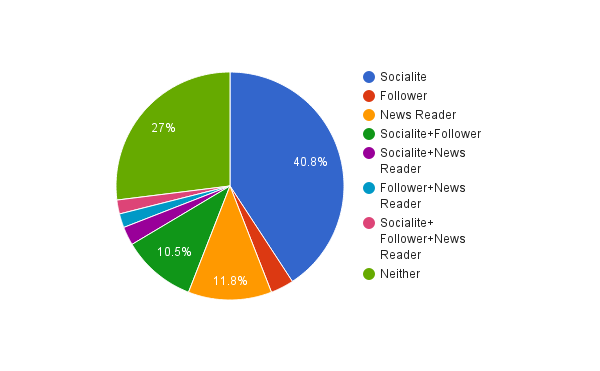
\includegraphics[scale=0.8]{images/usermodelChart.png}
  \captionof{figure}{Welcome screen}
\end{center}

\section{User Interface}

A typical user that uses our app will first be welcomed with a welcome screen as shown in the figure below.

\begin{center}
  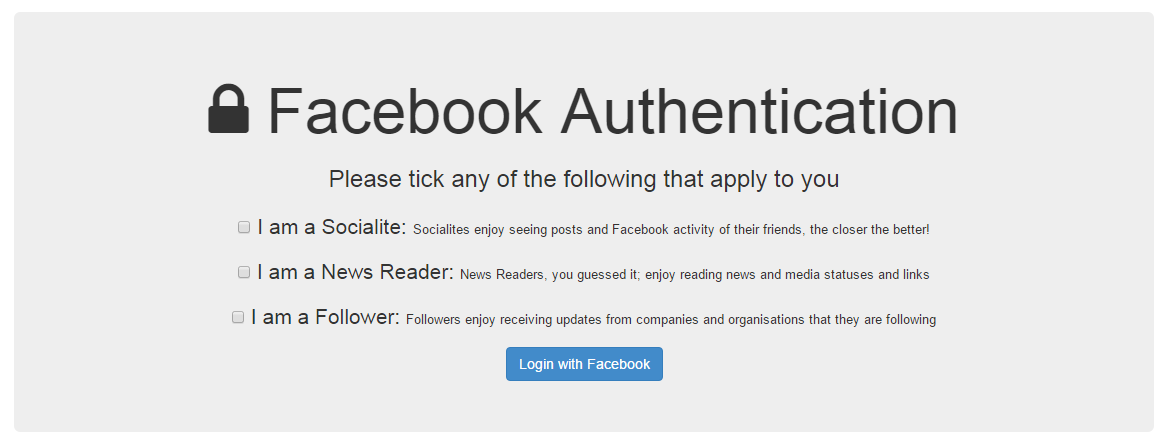
\includegraphics[scale=0.5]{images/mainscreen.png}
  \captionof{figure}{Welcome screen}
\end{center}

The user can choose one or more of the options before they click log in. When the log in is clicked, the user is taken to a typical log in screen from Facebook.

After logging in, the user will be able to see a Facebook feed.

\begin{center}
  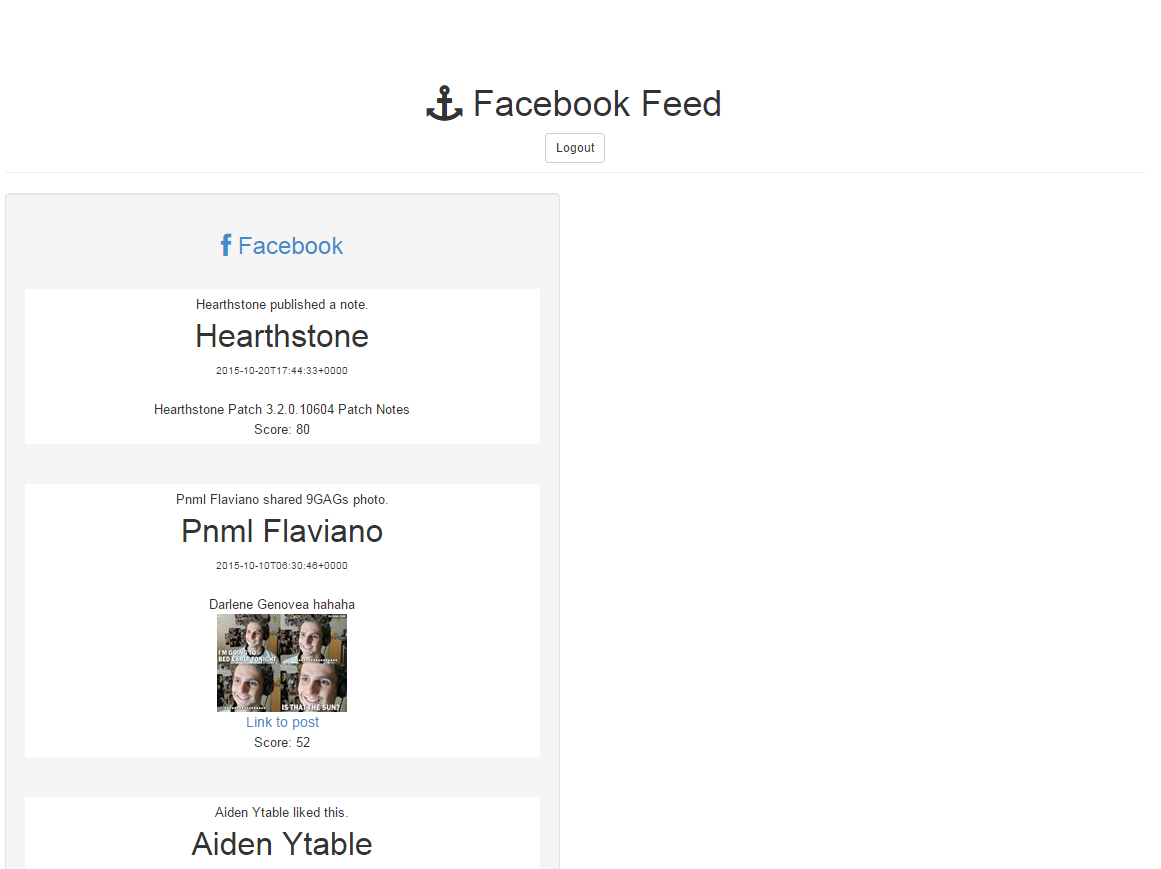
\includegraphics[scale=0.5]{images/rankedFeed.png}
  \captionof{figure}{Welcome screen}
\end{center}

The user interface is not the main focus of this thesis so it definitely could be improved. (Should i say this?)

\section{Problems Encountered}

\begin{itemize}
  	\item Facebook API Limitations
	\item Paging
	\item Asynchronous vs Synchronous
\end{itemize}

A typical user receives an enourmous amount of items to their feed daily. This means that we would be required to pull a large amount of feed items in order to decide which items that the user would prefer to see. Unfortunately Facebook has a limitation on how many API calls can be made in a period of time. Only 600 API calls can be made every 10 minutes. This limitation has prevented us from getting more data about the user such as searching through the feed to see if a friend has liked a particular post. Another limitation of the Facebook API involved the friends list. The Facebook API only allows us to get friends who have also installed the app. For our particular time frame, this is very impractical. Facebook API also does not show us how close the friends are to the user.  

